
\chapter{Motion in Two or Three Dimensions}

\section{Discussion Questions}

% 3.1
\discussion{As there is no velocity at the end of the swing the only force acting on the pendulum is gravity. A the midpoint the only, acceleraton would be towards the ``center'' of the rope.}

% 3.2
\discussion{It turns, the speed would initially increase as the vectors are orthogonal.}

% 3.3
\discussion{Never parallel, perpendicular at the top.}

% 3.4
\discussion{
(a) Stays the same (unless floor curves) \\
(b) Twice the distance \\
(c) Same
}

% 3.5
\discussion{Same as $\Delta{\vec{x}}$ is same, total distance is not same.}

% 3.6
\discussion{Hit at the same time, thrown will have greater speed.}

% 3.7
\discussion{Unclear what they are asking.}

% 3.8
\discussion{Problem is not stated very clearly, assume $v_x = v_y$. $\Delta{y} = \frac{1}{2}\frac{v_0^2}{g}$}

% 3.9
\discussion{
$\vec{v} = \left<v_{0_x},0\right>$, speed = $v_{0_x}$, $\vec{a} = \acceleration{\left<0, -9.8\right> }$
}

% 3.10
\discussion{Average velocity and average acceleration is 0.}

% 3.11
\discussion{$\sqrt{2}\cdot{}10$}

% 3.12
\discussion{$\vec{v}(t) = \velocity{\left<10,10*t\right>}$, $\vec{v}(5) = \velocity{51}$, $\Delta{x} = \distance{123}$}

% 3.13
\discussion{The car is moving forward, therefore the raindrops ``smear'' against the window.  For the windshield it would require the wind as only the vertical streaks would form. The best mathematical explanation I can think of is that the ``smears'' appear when the raindrop and car velocities are not parallel.}

% 3.14
\discussion{TODO: Review.  The dot product of the velocities of the wind and rain.}

% 3.15
\discussion{Straight across if you just want to be on the other side.  If you want to be directly across from the spot you are you would need to swim at an angle against the flow of the river.}

% 3.16
\discussion{It would be (d).  It would start slowing down, then hit it's maximum height and the speed would be equal to $v_{0_x}$, then the speed would start increasing as gravity pulls it downward.}

\section{Exercises}

\subsubsection*{Position and Velocity Vectors}
% 3.1
\exercise{
(a) $\velocity{\vT{1.5}{1.2}}$ \\
(b) \velocity{1.9} $\ang{-39}$
}

% 3.2
\exercise{
(a) $\distance{\vT{-50}{54}}$ \\
(b) $\distance{74}$
}

\begin{figure}[!ht]
    \centering
    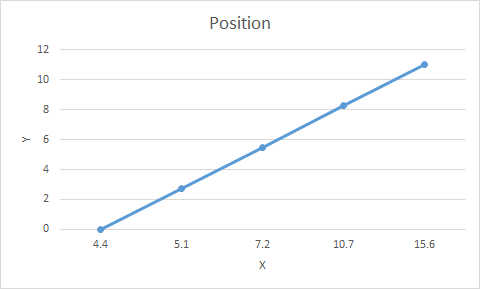
\includegraphics[scale=0.5]{mechanics/chapter3/problem3.3.png}
    \caption{Problem 3.3}
    \label{fig:Problem3.3}
\end{figure}

% 3.3
\exercise{
(a) $\acceleration{\vT{5.6}{5.5}}$ \\
(b) $\vec{v}(0) = \velocity{\vT{0.0}{5.5}}$, $\vec{v}(1) = \velocity{\vT{5.6}{5.5}}$, $\vec{v}(2) = \velocity{\vT{11.2}{5.5}}$ \\
(c) $\Fig{fig:Problem3.3}$ shows the position over time.
}

% 3.4
\exercise{
(a) $\vec{v}(t) = \velocity{\vT{0.280}{0.057t^2}}$ \\
(b) $\distance{4.26}$ \\
(c) $\velocity{1.88}, \ang{87.9}$
}

\subsubsection*{The Acceleration Vector}

\begin{figure}[!ht]
    \centering
    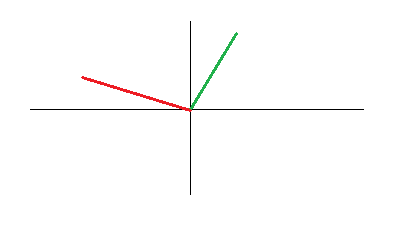
\includegraphics[scale=0.5]{mechanics/chapter3/problem3.5.png}
    \caption{Problem 3.5}
    \label{fig:Problem3.5}
\end{figure}

% 3.5
\exercise{
(a) $\Fig{fig:Problem3.5}$ \\
(b) $\acceleration{\vT{-8.77}{-2.67}}$ \\
(c) $\acceleration{9.16}, \ang{197}$
}

\begin{figure}[!ht]
    \centering
    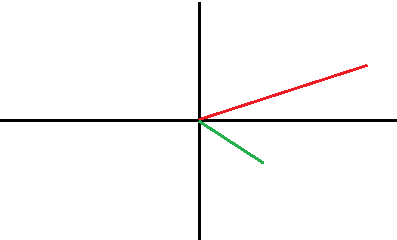
\includegraphics[scale=0.5]{mechanics/chapter3/problem3.6.png}
    \caption{Problem 3.6}
    \label{fig:Problem3.6}
\end{figure}


% 3.6
\exercise{
(a) $\velocity{\vT{}9.46{2.34}}$ \\
(b) $\velocity{9.74}, \ang{13.9}$ \\
(c) $\Fig{fig:Problem3.6}$
}

% 3.7
\exercise{
(a)TODO: Excel \\
(b) $\vec{v}(t) = \velocity{\vT{\alpha}{-2\beta{t}}}, \vec{a}(t) = \acceleration{\vT{0}{-2\beta}}$ \\
(c) $\vec{v}(2) = \velocity{\vT{2.4}{-4.8}}, \vec{a}(2)= \vT{0}{-2.4}$ \\
(d) TODO: Excel, Increasing, turning right
}

% 3.8
\exercise{
(a) $\vec{a}(t) = \acceleration{\vT{-0.036t}{0.550}}$ \\
(b) $\velocity{7.11}, \ang{35.7}$ \\
(c) $\acceleration{0.60}, \ang{336}$
}

\subsubsection{Projectile Motion}

% 3.9
\exercise{
(a) $\distance{0.502}$ \\
(a) $\distance{0.448}$ \\
(a) $\velocity{1.40}{-3.14}$ \\
(d) TODO
}

% 3.10
\exercise{$\velocity{1.30}$}

% 3.11
\exercise{\si{\centi\meter}}

% 3.12
\exercise{
(a) $\seconds{1.730}$ \\
(b) $\distance{14.7}$ \\
(c) $\seconds{1.73}$ \\
(d) $\distance{74.4}$ \\
(e) TODO
}

% 3.13
\exercise{
(a) $\velocity{28.6}$ \\
(b) $\velocity{34.6}$
}

% 3.14
\exercise{
(a) $\velocity{\vT{2.12}{3.3}}$ \\
(b) $\distance{7.34}$
}

% 3.15
\exercise{
$\acceleration{72.5}$
}

% 3.16
\exercise{
(a) $\velocity{\vT{39.8}{58.8}}$ \\
(b) $\seconds{6}$ \\
(c) $\distance{176}$ \\
(d) $\distance{239}$ \\
(e) $\vec{a_h} = \acceleration{\vT{0,-9.8}}$, $\vec{v_h} = \acceleration{\vT{39.8,}}$
}

% 3.17
\exercise{
(a) $t = \seconds{1.22}, \seconds{7.14}$ \\
(b) $\vec{v}(1.22) = \velocity{\vT{31.5}{8.54}}, \vec{v}(7.14) = \velocity{\vT{31.5}{-8.54}}$ \\
(a) $\velocity{33.0}, \ang{-38.5}$
}

% 3.18
\exercise{
(a) $\vec{a} = \acceleration{\vT{0}{-8.97}}$ \\
(b) $\vec{v_0} = \velocity{\vT{7.55}{9.33}}, \vec{v_f} = \velocity{\vT{7.55}{-9.33}}$ \\
(c) $\distance{15.7}$ \\
(d) Because g is a fixed value, it should be the current acceleration. \\
(e) TODO
}

% 3.19
\exercise{
(a)  $D = \distance{1.53}$ \\
(b)  $V = \velocity{-0.886}$
}

% 3.20
\exercise{
(a) $\ang{53.1}$ \\
(b) $\vec{a} \ \acceleration{\vT{0}{-9.8}}, \vec{v} \ \velocity{\vT{16}{0}}$ \\
(c) $\distance{15.9}$, $\velocity{18.6}$
}

% 3.21
\exercise{
(a) $\distance{12.9}$ \\
(b) $\distance{29.0}$ \\
(c) $\distance{39.3}$ \\
(d) TODO
}

% 3.22
\exercise{
(a) $\distance{288}$  \\
(b) $\distance{90.4}$ \\
(c) $\distance{90.4}$ \\
(b) $\vec{v_B} = \velocity{\vT{19.6}{-74.5}}, \vec{v_G} = \velocity{\vT{19.6}{100}}$
}

\subsubsection*{Motion in a Circle}

% 3.23
\exercise{
(a) $\acceleration{0.0337}, 0.00344$ \\
(b) $\hours{1.41}$
}

% 3.24
\exercise{$\acceleration{21.6}$}

% 3.25
\exercise{$\velocity{130}$}

% 3.26
\exercise{
(a) $\velocity{11.8}$ \\
(b) 9.47g
}

% 3.27
\exercise{
This problem seems to be ignoring gravity, or I don't understand something. Even an online article~\footnote{https://www.real-world-physics-problems.com/ferris-wheel-physics.html} says different. \\
(a) $\acceleration{3.63}$ upwards\\
(b) $\acceleration{3.63}$ downwards\\
(c) $\seconds{12.3}$
}

% 3.28
\exercise{
(a) $\velocity{2.98\cdot{}10^3}$ \\
(b) $\acceleration{5.95\cdot{}10^{-3}}$ \\
(c) $\velocity{4.78\cdot{}10^4}$, $\acceleration{3.95\cdots{}10^{-2}}$
}

% 3.29
\exercise{
(a) 12.5g   \\
(b) 2.83g   \\
(c) 255.5 rev/min
}

\subsubsection*{Relative Velocity}

% 3.30
\exercise{
(a) $\velocity{5.0}$ \\
(a) $\velocity{-16.0}$ \\
(a) $\velocity{-13.0}$
}

% 3.31
\exercise{
(a) $\seconds{10}$ \\
(b) $\seconds{110}$
}

% 3.32
\exercise{
 (4) $\seconds{2.75}$ \\
 (2.8) $\seconds{3.86}$
 
}

% 3.33
\exercise{$\velocity{0.42}, \ang{43}$
}

% 3.34
\exercise{TODO}

% 3.35
\exercise{
(a) $\velocity{4.9}, \ang{-16}$ \\
(b)$\seconds{210}$ \\
(c) $\distance{540}$
}

% 3.36
\exercise{
(a) $\velocity{\vT{4.2}{2.5}}$ \\
(b) $\velocity{4.9}, \ang{16}$ \\
(c) $\seconds{210}$
}

% 3.37
\exercise{
(a) $\ang{-120}$ \\
(b) $\hours{6.25}$
}

% 3.38
\exercise{
(a) $\ang{167}$ \\
(b) TODO
}

\section{Problems}

\section{Challenge Problems}
